% Impostazioni principali
\documentclass[t, compress, hyperref={pdfpagelabels=false}]{beamer}
\usefonttheme[onlymath]{serif}


%         ----------------------------------------------         %
%        /                                              \        %
%--------               START PREAMBLE                   --------%
%        \                                              /        %
%         ----------------------------------------------         %

% Titolo che appare nella prima slide del documento
\newcommand{\titolo}{Generalized Linear Models (GLM)}
\newcommand{\sottotitolo}{}

% Titolo che appare nella barra in basso di ogni slide, al centro
% Sono due variabili:
% * una puo' essere utilizzata per l'intero corso. Se impostata nel preambolo sovrascrive quella di seguito.
% * l'altra puo' identificare ciascun documento
\newcommand{\titolocompleto}{Statistics Course - }
\newcommand{\titoloshort}{\titolo}

% Numero di capitolo o altro nome che appare in basso di ogni slide, vicino al numero di pagina
\newcommand{\numerocapitolo}{Chapter 13}

% Include il documento che contiene il preambolo

%%%%%%%%%%%%%%%%%%%%%%%%%%%%%%%%%%%%%%%%%%%%%%%%%%%%%%%%%%%%%%%%%%%%%%%%%%%%%%
%%%%%%%%%%%%%%%%%%%%%%%%%%%% VARIABILI DA DEFINIRE %%%%%%%%%%%%%%%%%%%%%%%%%%%
%%%%%%%%%%%%%%%%%%%%%%%%%%%%%%%%%%%%%%%%%%%%%%%%%%%%%%%%%%%%%%%%%%%%%%%%%%%%%%

% Titolo che appare nella barra in basso di ogni slide, al centro
% Se impostato ha la precedenza rispetto a quello di ogni singola slide

%\renewcommand{\titolocompleto}{}

% non c'e' newcommand{\sottotitolo} perche' viene definito in ogni slide
\newcommand{\data}{}



%%%%%%%%%%%%%%%%%%%%%%%%%%%%%%%%%%%%%%%%%%%%%%%%%%%%%%%%%%%%%%%%%%%%%%%%%%%%%%
%%%%%%%%%%%%%%%%%%%%%%%%%%%%%%%%%% PACKAGES %%%%%%%%%%%%%%%%%%%%%%%%%%%%%%%%%%
%%%%%%%%%%%%%%%%%%%%%%%%%%%%%%%%%%%%%%%%%%%%%%%%%%%%%%%%%%%%%%%%%%%%%%%%%%%%%%
\usepackage[latin1]{inputenc}   
\usepackage{graphicx}
\usepackage{rotating}
\usepackage{rotfloat}
\usepackage{color}
\usepackage{colortbl}
\usepackage{../includeTex/floatflt}
\usepackage{tikz}
\usepackage{hyperref}
\usepackage{pgfpages} 
\usepackage{ifthen}
\usepackage{wasysym}
\usepackage{multirow}



%%%%%%%%%%%%%%%%%%%%%%%%%%%%%%%%%%%%%%%%%%%%%%%%%%%%%%%%%%%%%%%%%%%%%%%%%%%%%%
%%%%%%%%%%%%%%%%%%%%%%%%%%%% IMPOSTAZIONI GENERALI %%%%%%%%%%%%%%%%%%%%%%%%%%%
%%%%%%%%%%%%%%%%%%%%%%%%%%%%%%%%%%%%%%%%%%%%%%%%%%%%%%%%%%%%%%%%%%%%%%%%%%%%%%

% Beamer theme
%\usetheme{CambridgeUS}      
\usetheme{Madrid}      

% Immagini da visualizzare
\newcommand{\materiale}{minitab}

% Path delle immagini
\graphicspath{{../images/}}

% Per caricare le formule matematiche con il giusto font 
% Questo sostituisce l'opzione mathserif di documentclass (obsoleta) 
\usefonttheme[onlymath]{serif}      

     

%%%%%%%%%%%%%%%%%%%%%%%%%%%%%%%%%%%%%%%%%%%%%%%%%%%%%%%%%%%%%%%%%%%%%%%%%%%%%%
%%%%%%%%%%%%%%%%%%%%%%%%%%%%%%%%%%% COLORI %%%%%%%%%%%%%%%%%%%%%%%%%%%%%%%%%%%
%%%%%%%%%%%%%%%%%%%%%%%%%%%%%%%%%%%%%%%%%%%%%%%%%%%%%%%%%%%%%%%%%%%%%%%%%%%%%%

\definecolor{grigio}{rgb}{0.46,0.48,0.48}
\definecolor{giallo}{rgb}{1,0.84,0}
\definecolor{coolred}{rgb}{0.83,0.06,0.27}
\definecolor{arancio}{rgb}{0.97,0.46,0.09}
\definecolor{verde}{rgb}{0.25,0.78,0.25}
\definecolor{qblu}{rgb}{0.24,0.27,0.74}
\definecolor{azzurro}{rgb}{0.37,0.91,0.90}

\definecolor{grigio}{rgb}{0.46,0.48,0.48}
\definecolor{blu}{rgb}{0.25,0.28,0.78}

\definecolor{sfondoScopo}{rgb}{0.75,0.785,0.83}
\definecolor{darkred}{named}{qblu}
\definecolor{blue}{named}{qblu}

\setbeamercolor{scopo}{bg=sfondoScopo}
\setbeamercolor{section in toc}{fg=black,bg=white}
\setbeamercolor{alerted text}{fg=darkred!80!gray}
\setbeamercolor{palette primary}{fg=darkred!60!black,bg=gray!30!white}
\setbeamercolor{palette secondary}{fg=darkred!70!black,bg=gray!15!white}
\setbeamercolor{palette tertiary}{bg=darkred!80!black,fg=gray!10!white}
\setbeamercolor{palette quaternary}{fg=darkred,bg=gray!5!white}

\setbeamercolor{sidebar}{fg=darkred,bg=gray!15!white}
\setbeamercolor{palette sidebar primary}{fg=darkred!10!black}
\setbeamercolor{palette sidebar secondary}{fg=white}
\setbeamercolor{palette sidebar tertiary}{fg=darkred!50!black}
\setbeamercolor{palette sidebar quaternary}{fg=gray!10!white}

\setbeamercolor{titlelike}{parent=pallette primary,fg=darkred}
\setbeamercolor{frametitle}{bg=gray!10!white}
\setbeamercolor{frametitle right}{bg=gray!60!white}

\setbeamercolor{separation line}{}
\setbeamercolor{fine separation line}{}

%% Definizione dei colori da assegnare ai box
\setbeamercolor{postit}{fg=white,bg=qblu}
\setbeamercolor{postut}{fg=qblu,bg=gray!60!white}

%% Definizione dei colori per i diagrammi
\definecolor{bloccoIniziale}{rgb}{0.94,0.93,0.48}
\definecolor{bloccoFinale}{rgb}{0.86,0.25,0.27}
\definecolor{blocco}{rgb}{0.56,0.58,0.77}
\definecolor{bloccoSospeso}{rgb}{0.94,0.81,0.36}



%%%%%%%%%%%%%%%%%%%%%%%%%%%%%%%%%%%%%%%%%%%%%%%%%%%%%%%%%%%%%%%%%%%%%%%%%%%%%%
%%%%%%%%%%%%%%%%%%%%%%%%% STRUTTURA DELLE DIAPOSITIVE %%%%%%%%%%%%%%%%%%%%%%%%
%%%%%%%%%%%%%%%%%%%%%%%%%%%%%%%%%%%%%%%%%%%%%%%%%%%%%%%%%%%%%%%%%%%%%%%%%%%%%%

% Intestazione
\setbeamertemplate{headline}
{
  \leavevmode%
  \hbox{%
  \begin{beamercolorbox}[wd=.5\paperwidth,ht=2.25ex,dp=1ex,right]{section in head/foot}%
    \usebeamerfont{section in head/foot}\insertsectionhead\hspace*{2ex}
  \end{beamercolorbox}%
  \begin{beamercolorbox}[wd=.5\paperwidth,ht=2.25ex,dp=1ex,left]{subsection in head/foot}%
    \usebeamerfont{subsection in head/foot}\hspace*{2ex}\insertsubsectionhead
  \end{beamercolorbox}}%
  \vskip0pt%
}

% Pie' di pagina
\setbeamertemplate{footline}
{
  \hbox{%
    \begin{beamercolorbox}[wd=.20\paperwidth, ht = 2.25ex, dp = 1ex, center]{palette sidebar secondary}%
      \usebeamerfont{author in head/foot}%\insertshortauthor~~(\insertshortinstitute) 
      
\includegraphics[width=1.5cm]{QUANTIDE.jpg}
    \end{beamercolorbox}%
    \begin{beamercolorbox}[wd=.57\paperwidth, ht = 2.25ex, dp = 1ex, center]{title in head/foot}%
      \usebeamerfont{title in head/foot}{\titolocompleto \titoloshort}
    \end{beamercolorbox}%
    \begin{beamercolorbox}[wd=.13\paperwidth, ht = 2.25ex, dp = 1ex, left]{date in head/foot}%
      \hspace*{0.4em} \usebeamerfont{date in head/foot} {\numerocapitolo}
    \end{beamercolorbox}%
    \begin{beamercolorbox}[wd=.10\paperwidth, ht = 2.25ex, dp = 1ex, right]{date in head/foot}%
       \usebeamerfont{date in head/foot} \insertframenumber{} / \inserttotalframenumber \hspace*{2ex} 
    \end{beamercolorbox}%
  }%
  \vskip0pt%
}



%%%%%%%%%%%%%%%%%%%%%%%%%%%%%%%%%%%%%%%%%%%%%%%%%%%%%%%%%%%%%%%%%%%%%%%%%%%%%%
%%%%%%%%%%%%%%%%%%%%%%%%%%% STILE DELLE DIAPOSITIVE %%%%%%%%%%%%%%%%%%%%%%%%%%
%%%%%%%%%%%%%%%%%%%%%%%%%%%%%%%%%%%%%%%%%%%%%%%%%%%%%%%%%%%%%%%%%%%%%%%%%%%%%%

% Simboli di navigazione
\setbeamertemplate{navigation symbols}{}

% Modifica lo stile dell'elenco (di primo livello)
\useitemizeitemtemplate{$\star$} % Usa la stella

% Interlinea (fattore di scala; NON e' un valore assoluto)
\renewcommand{\baselinestretch}{1.2}  

% Definisci stile per vettori e matrici
\newcommand{\vect}[1]{\boldsymbol{\underline{#1}}} % Grassetto e sottolineato
\newcommand{\matr}[1]{\boldsymbol{#1}} % Grassetto

% Definire stile per valore assoluto
\providecommand{\abs}[1]{\lvert#1\rvert}
\providecommand{\norm}[1]{\lVert#1\rVert}

% Cambiare il nome delle figure e delle tabelle
\renewcommand{\figurename}{Figura}
\renewcommand{\tablename}{Tabella}

% Definizione sezioni, ecc.
\newcommand{\livelloA}{\section}
\newcommand{\livelloB}{\subsection}
\newcommand{\livelloC}{\subsubsection}

% Livello di profondita' del 'content panel' del PDF
% \hypersetup{bookmarksdepth=4} % il valore di default va bene

% Definizione prima slide
\title{\textbf{\titolo}}
\author{\sottotitolo}
\date{\data}






%         ----------------------------------------------         %
%        /                                              \        %
%--------               START DOCUMENT                   --------%
%        \                                              /        %
%         ----------------------------------------------         %

\begin{document}

% Pagina del titolo
\frame{\titlepage}

% Indice
% \begin{frame}
% 	 \tableofcontents
% \end{frame}

% Documento
% I soli contenuti del documento sono in un file esterno. Questo semplifica enormemente le cose qualora si volessero creare dei manuali (singoli documenti) a partire da diversi documenti.
\livelloA{Linear Model (LM)}

\livelloB{Introduction: smoothing}

\begin{frame}
  \begin{itemize}
    \item Regression is the study of the change of the distribution of one variable, $ y $, according to the value of another variable, $ x $.
    \item Both continous and discrete variables can be included in regression problems.
    \item Formally, a relationship between $ x $ and $ y $ usually means that the expected value of $ y $ is different for different values of $ x $.
    \item At this stage, changes in $ \sigma^2 $ or other aspects of the distribution are not considered.
    \item When $ y $ is continous, changes in $ y $ are smooth (continuous and differentiable), and the model used is:
      $$ E(y|x) = g(x) $$
      for some unknown smooth function $ g(\cdot) $.
  \end{itemize}
\end{frame}



\livelloB{Regression}

\begin{frame}
  \begin{itemize}
    \vspace{0.75cm}
    \item A variety of functions can be used to estimate $ g(\cdot) $. These functions are called \textbf{scatterplot smoother}.
    \vspace{1.25cm}
    \item For a pair $ (x_i, y_i) $, $ i = 1, \dots, n $:
      $$ y_i = g(x_i) + \varepsilon_i $$
      where $ g(\cdot) $ is called the \textbf{regression function}.
  \end{itemize}
\end{frame}



\livelloB{Regression: example 1}

\begin{frame}
  \begin{itemize}
    \vspace{0.25cm}
    \item A chemical theory suggests that the temperature at which a certain reaction occurs is 180$^\circ$.
    \vspace{0.25cm}
    \item The results of 10 indipendent experiments, contained in \texttt{reaction.dat}, are:\\
      179.4, 177.5, 180.6, 178.1, 180.2, 179.3, 180.0, 178.3, 179.1, 181.1.
    \vspace{0.25cm}
    \item In this example, $ n = 10 $ and
      $$ E(y_i) = \beta_0 \text{ for } i = 1, \dots, n $$
    \item More generally, however, different observations are associated with different experimental conditions or different values of one or more \textbf{explanatory variables} as the following examples will illustrate.
  \end{itemize}
\end{frame}



\livelloB{Regression: example 2}

\begin{frame}
  \begin{itemize}
    \vspace{0.2cm}
    \item To compare two growth hormones, 19 chicken were tested, 11 being assigned to hormone A and 8 to hormone B. 
    \vspace{0.2cm}
    \item The following were the gains in weight (grams) over the period of experiment, contained in \texttt{hormones.dat}:\\
      \vspace{0.2cm}
      \begin{footnotesize}
        \hspace{1cm} Hormone A: 615, 645, 840, 615, 365, 450, 450, 530, 756, 785, 560. \\
        \hspace{1cm} Hormone B: 870, 895, 1035, 700, 560, 756, 785, 980.       
      \end{footnotesize}
    \vspace{0.2cm}
    \item $ E(y_{ij}) = \beta_{i} $ for $ j = 1, \dots, n_i $; $ i = 1, 2 $.
    \vspace{0.2cm}
    \item Thus, $ \beta_{1} $ and $ \beta_{2} $ are the expectations of $ y $ for hormones A and B, respectively.
    \vspace{0.2cm}
    \item Typically, it is interesting in whether or not $ \beta_{1} = \beta_{2} $ or in the range of values for the difference $ \beta_{1} - \beta_{2} $.
  \end{itemize}
\end{frame}


\livelloB{Regression: example 3}

\begin{frame}
  \begin{itemize}
    \vspace{0.25cm}
    \item In an experiment to investigate the effects of a depressant drug, the reaction times of then male rats to a certain stimulus were measured after a specified dose of the drug have been administered to each rat.
    \vspace{0.25cm}
    \item The results, contained in \texttt{drug.dat}, were as follows:\\
      \vspace{0.2cm}
      \begin{tiny}
        \begin{tabular}{lcccccccccc}
          \hline
          Rat number: & 1 & 2 & 3& 4&5&6&7&8&9&10\\
          \hline
          Dose (mg): & 0.0&0.1&0.2&0.3&0.4&0.5&0.6&0.7&0.8&0.9\\
          Reaction time (secs): & 0.32&0.24&0.40&0.52&0.44&0.56&0.64&0.52&0.60&0.80\\
          \hline
        \end{tabular}       
      \end{tiny}
    \vspace{0.25cm}
    \item A simple model for this data might be a straight line, i.e.
      $$ E(y_i|x_i) = \beta_0 + \beta_1 x_i \text{  for } i = 1, \dots, n $$
    \item For simplicity, usually the above formula is written as $ E(y_i) = \beta_0 + \beta_1 x_i $, the conditioning on $ x_i $ being understood.
  \end{itemize}
\end{frame}



\livelloB{Regression: example 4}

\begin{frame}
  \begin{itemize}
    \vspace{0.25cm}
    \item In the study of the polyesterification of fatty acids with glycols, the effect of temperature ($ ^\circ $C) on the percentage conversion of the esterification process was investigated.
    \item The following data, contained in \texttt{polyesterification.dat}, are the results of an experiment using a catalyst of $ 4 \cdot 10^{-4} $ mole zinc chloride per 100 grams of fatty acid.
      \vspace{0.2cm}
      \begin{small}
        \begin{tabular}{lcccccc}
          \hline
          Temperature ($ ^\circ $C): & 175&200&225&250&275&300\\
          Percentage conversion (\%): & 67&83&93&97&99&92\\
          \hline
        \end{tabular}       
      \end{small}
    \vspace{0.25cm}
    \item This is similar to the previous example, but now a quadratic function of $x$ seems sensible:
      $$ E(y_i) = \beta_0 + \beta_1 x_1 + \beta_2 x_1^2 \text{  for } i = 1, \dots, n $$
  \end{itemize}
\end{frame}



\livelloB{Regression: example 5}

\begin{frame}
  \begin{itemize}
    \vspace{0.5cm}
    \item The data in the \texttt{oxidant.dat} file give levels of an air pollutant, ``Oxidant'', together with levels of four meteorological variables recorded on 30 days during one summer.
    \vspace{0.5cm}
    \item Which, if any, of the four indipendent variables seem to be related to levels of oxidant?
    \vspace{0.5cm}
    \item Again, a simple starting point would be:
      $$ E(y_i) = \beta_0 + \beta_1 x_1 + \beta_2 x_2 + \beta_3 x_3 + \beta_4 x_4 \text{  for } i = 1, \dots, n $$
  \end{itemize}
\end{frame}



\livelloB{Linear model formulae and functions in R}

\begin{frame}
  Model formulae\\
  \begin{center}
    \begin{footnotesize}
      \begin{tabular}{ll}
        \hline
        Expression & Description \\
        \hline
        \texttt{y }$\sim$\texttt{ x}                         & Simple regression \\
        \texttt{y }$\sim$\texttt{ 1 + x}                     & Explicit intercept \\
        \texttt{y }$\sim$\texttt{ -1 + x}                    & Through the origin \\
        \texttt{y }$\sim$\texttt{ x + x\^{ }2}               & Quadratic regression \\
        \texttt{y }$\sim$\texttt{ x1 + x2 + x3}              & Multiple regression \\
        \texttt{y }$\sim$\texttt{ G + x1 + x2}               & Parallel regressions \\
        \texttt{y }$\sim$\texttt{ G / (x1 + x2)}             & Separate regressions \\
        \texttt{sqrt(y) }$\sim$\texttt{ x + x\^{ }2}         & Transformed \\
        \texttt{y }$\sim$\texttt{ G}                         & Single classification \\
        \texttt{y }$\sim$\texttt{ A + B}                     & Randomized block \\
        \texttt{y }$\sim$\texttt{ B + N * P}                 & Factorial in blocks \\
        \texttt{y }$\sim$\texttt{ x + B + N * P}             & with covariate \\
        \texttt{y }$\sim$\texttt{ . -x1}                     & All variables except \texttt{x1} \\
        \texttt{y }$\sim$\texttt{ . + A:B}                   & Add interaction (\texttt{update}) \\
        \texttt{Nitrogen }$\sim$\texttt{ Times*(River/Site)} & More complex design \\ 
        \hline
      \end{tabular}   
    \end{footnotesize}
  \end{center}
\end{frame}

\begin{frame}
  \vspace{0.5cm}
  Common R functions for inference
  \vspace{0.25cm}
  \begin{center}
    \begin{tabular}{ll}
      \hline
      Expression & Description \\
      \hline
      \texttt{coef(obj)} & regression coefficients \\
      \texttt{resid(obj)} & residuals \\
      \texttt{fitted(obj)} & fitted values \\
      \texttt{summary(obj)} & analysis summary \\
      \texttt{predict(obj, newdata = ndat)} & predict for newdata \\
      \texttt{deviance(obj)} & residual sum of squares\\
      \hline
    \end{tabular} 
  \end{center}
\end{frame}



\livelloB{Linear model}

\begin{frame}
  \begin{itemize}
    \vspace{0.5cm}
    \item All the examples discussed above can be expressed in the form:
      $$ E(y_i) = \beta_0 + \displaystyle\sum_{j=1}^p \beta_j x_{i,j} $$
    \vspace{0.5cm}
    \item The above formula can be rewritten as
      $$ \vect{\mu} = E(\vect{y}) = \matr{X} \vect{\beta} $$
      where $ \matr{X} $ is a $ n \text{ x } (p+1) $ matrix, with all ones in the first columns, and $ \vect{\beta} $ is the vector of $ \beta_0, \beta_1, \dots, \beta_p $.
  \end{itemize}
\end{frame}

\begin{frame}
  \begin{itemize}
    \vspace{0.5cm}
    \item In the example 1: $ \matr{X} = (\vect{1}) $ and $ \vect{\beta} = (\beta_0) $
    \vspace{0.5cm}
    \item In the example 2: 
      $$ 
        \matr{X} = 
        \left(
          \begin{array}{cc} 
            1 & 0 \\
            \vdots & \vdots \\
            1 & 0 \\
            0 & 1 \\
            \vdots & \vdots \\
            0 & 1 \\  
          \end{array}
        \right)_{n\text{x}2}
        \vect{\beta} =
        \left(
          \begin{array}{c} 
            \beta_1 \\
            \beta_2 \\
          \end{array}
        \right)_{2\text{x}1}
      $$
  \end{itemize}
\end{frame}

\begin{frame}
  \begin{itemize}
    \vspace{0.5cm}
    \item In the example 3: 
      $$ 
        \matr{X} = 
        \left(
          \begin{array}{cc} 
            1 & x_1 \\
            \vdots & \vdots \\
            1 & x_n \\
          \end{array}
        \right)_{n\text{x}2}
        \vect{\beta} =
        \left(
          \begin{array}{c} 
            \beta_0 \\
            \beta_1 \\
          \end{array}
        \right)_{2\text{x}1}
      $$
    \vspace{0.5cm}
    \item In the example 4: 
      $$ 
        \matr{X} = 
        \left(
          \begin{array}{ccc} 
            1 & x_1 & x_1^2\\
            \vdots & \vdots & \vdots \\
            1 & x_n & x_n^2\\
          \end{array}
        \right)_{n\text{x}3}
        \vect{\beta} =
        \left(
          \begin{array}{c} 
            \beta_0 \\
            \beta_1 \\
            \beta_2
          \end{array}
        \right)_{3\text{x}1}
      $$
  \end{itemize}
\end{frame}

\begin{frame}
  \begin{itemize}
    \vspace{0.5cm}
    \item In the example 5: 
      $$ 
        \matr{X} = 
        \left(
          \begin{array}{ccccc} 
            1 & x_{1,1} & x_{1,2} & x_{1,3} & x_{1,4}\\
            \vdots & \vdots & \vdots & \vdots & \vdots\\
            1 & x_{n,1} & x_{n,2} & x_{n,3} & x_{n,4}\\
          \end{array}
        \right)_{n\text{x}5}
        \vect{\beta} =
        \left(
          \begin{array}{c} 
            \beta_0 \\
            \beta_1 \\
            \beta_2 \\
            \beta_3 \\
            \beta_4 \\
          \end{array}
        \right)_{3\text{x}1}
      $$
    \vspace{0.5cm}
    \item Models of the form $ \mu = E(y_i) = \matr{X}\beta $ are called \textbf{linear models}, because they are linear in the \textbf{unknown parameters} comprising the elements of $ \beta $.
  \end{itemize}
\end{frame}


\livelloB{Regression: example 6}

\begin{frame}
  \begin{itemize}
    \item The file \texttt{hotdogs.dat} contains calories and sodium data for three types of hot dogs: Poultry, Beef, Meat.
    \vspace{0.25cm}
    \item 20 Beef, 17 Meat and 17 Poultry hot dogs. These data may be thinked as samples from much larger populations.
    \vspace{0.25cm}
    \item Looking at the density estimates it seems reasonable, at least as a first approximation, to model the distribution as Normal.
    \vspace{0.25cm}
    \item The following model can be adopted (model 1):
      $$ B_1, \dots, B_{20} \sim \text{i.i.d. } N(\mu_B, \sigma) $$
      $$ M_1, \dots, M_{17} \sim \text{i.i.d. } N(\mu_M, \sigma) $$
      $$ P_1, \dots, P_{17} \sim \text{i.i.d. } N(\mu_P, \sigma) $$
  \end{itemize}
\end{frame}

\begin{frame}
  \begin{itemize}
    \vspace{0.75cm}
    \item An equivalent formulation (model 2):
      $$ B_1, \dots, B_{20} \sim \text{i.i.d. } N(\mu, \sigma) $$
      $$ M_1, \dots, M_{17} \sim \text{i.i.d. } N(\mu+\delta_M, \sigma) $$
      $$ P_1, \dots, P_{17} \sim \text{i.i.d. } N(\mu+\delta_P, \sigma) $$
    \vspace{0.75cm}
    \item There are three parameters for the population means and one for the standard deviation.
  \end{itemize}
\end{frame}

\begin{frame}
  \vspace{1cm}
  \begin{table}
    \begin{tabular}{cccc}
      \hline
      \textbf{Model 1} & \textbf{Model 2} & \textbf{Interpretation} & \textbf{Approx value}\\
      \hline
      $ \mu_B $          & $ \mu $            & MCC of Beef hot dogs    & 157 \\
      $ \mu_M $          & $ \mu + \delta_M $ & MCC of Meat hot dogs    & 159 \\
      $ \mu_P $          & $ \mu + \delta_P $ & MCC of Poultry hot dogs & 119 \\
      $ \mu_M - \mu_B $  & $ \delta_M $       &                                          &   2 \\
      $ \mu_P - \mu_B $  & $ \delta_P $       &                                          & -38 \\
      $ \sigma $         & $ \sigma $         & Standard deviation                       &  29 \\
      \hline
    \end{tabular}
  \end{table}
MCC: Mean calorie content
\end{frame}

\begin{frame}
  \begin{itemize}
    \vspace{0.25cm}
    \item Rewriting the data matrix in a slightly different form reveals some mathematical structure common to many models.
    \vspace{0.25cm}
    \item Let $ (y_1, \cdot, y_{54}) $ be the calorie contents. Two new variables are defined:
      $$
        x_{1,i} = \left\{ 
        \begin{array}{ll}
          1 & \text{if the }i\text{-th hot dog is Meat} \\
          0 & \text{otherwise} \\
        \end{array} \right.
      $$
      $$
        x_{2,i} = \left\{ 
        \begin{array}{ll}
          1 & \text{if the }i\text{-th hot dog is Poultry} \\
          0 & \text{otherwise} \\
        \end{array} \right.
      $$
    \vspace{0.25cm}
    \item $ x_{1,i} $ and $ x_{2,i} $ are indicator or dummy variables.
    \vspace{0.25cm}
    \item If there are $ k $ populations, then $ k-1 $ indicators suffice.
  \end{itemize}
\end{frame}

\begin{frame}
  \begin{itemize}
    \item Model 2 can be stated as
      $$ y_i = \mu + \delta_M x_{1,i} + \delta_P x_{2,i} + \varepsilon_i $$
      $$ \varepsilon_1, \cdot, \varepsilon_{54} \sim \text{i.i.d. } N(0, \sigma) $$
    \item Let
  \end{itemize}
  \vspace{0.25cm}
  \begin{columns}[l]
    \column{0.1\textwidth}
    \column{0.4\textwidth}
      \vspace{0.5cm}
      $$ \vect{}y = (y_1, \cdot, y_{54})^T $$
      $$ \vect{\beta} = (\mu, \delta_M, \delta_P)^T $$
      $$ \vect{\varepsilon} = (\varepsilon_1, \cdot, \varepsilon_{54})^T $$
    \column{0.5\textwidth}
      \vspace{-1cm}   
      $$ 
        \matr{X} = 
       \left(
          \begin{array}{ccc} 
            1 & 0 & 0 \\
            \vdots & \vdots & \vdots \\
            1 & 0 & 0 \\
            0 & 1 & 0 \\
            \vdots & \vdots & \vdots \\
            0 & 1 & 0 \\
            0 & 0 & 1 \\
            \vdots & \vdots & \vdots \\
            0 & 0 & 1 \\  
          \end{array}
        \right)_{54\text{x}3}
      $$
  \end{columns}
\end{frame}



\livelloB{Deterministic and random part}

\begin{frame}
  \begin{itemize}
    \vspace{0.5cm}
    \item The general form of the linear model:
      $$ \vect{y} = \matr{X} \vect{\beta} + \vect{\varepsilon} $$
      or    
      $$ y_i = \beta_0 + \beta_1 \cdot x_{i1} + \beta_2 \cdot x_{i2} + \dots + \beta_p \cdot x_{ip} + \varepsilon_i $$
      or
      $$ y_i \sim N(\mu_i, \sigma) $$
      with $ \mu_i = \beta_0 + \sum_j \beta_j x_{j,i} $ and $ \varepsilon_i \sim \text{i.i.d. } N(0, \sigma) $.
    \vspace{0.5cm}
    \item This model has $ p +2 $ parameters: $ \beta_0, \beta_1, \dots, \beta_p, \sigma $.
  \end{itemize}
\end{frame}

\begin{frame}
  \begin{itemize}
    \vspace{0.5cm}
    \item $ \matr{X}\vect{\beta} = \vect{\mu} $: \textbf{systematic} part, \textbf{deterministic} part or \textbf{signal}. %It represents the explanaible differences between populations.
    \vspace{0.5cm}
    \item $ \vect{\varepsilon} $: \textbf{random} or \textbf{noise} component.
    \vspace{0.5cm}
    \item response $ = $ signal $ + $ noise
    \vspace{0.5cm}
    \item Models in which the signal is a linear function of parameters ($ \mu $, $ \delta_M $, $ \delta_P $ in the example) and response is a linear function of signal and noise, are linear models.
  \end{itemize}
\end{frame}



\livelloB{Maximum Likelihood Estimate}

\begin{frame}
  \begin{itemize}
    \vspace{0.5cm}
    \item The likelihood function is
     \begin{footnotesize}
       $$
          \begin{array}{rl} 
            l(\beta_0, \dots, \beta_p, \sigma) & = \displaystyle\prod_{i=1}^n p(y_i|\beta_0, \dots, \beta_p, \sigma) = \\  
            & = \displaystyle\prod_{i=1}^n \frac{1}{\sqrt{2\pi\sigma}} \exp{\left(-\frac{1}{2}\left(\frac{y_i-\mu_i}{\sigma}\right)^2\right)} = \\
            & = \displaystyle\prod_{i=1}^n \frac{1}{\sqrt{2\pi\sigma}} \exp{\left(-\frac{1}{2}\left(\frac{y_i-(\beta_0+\sum_j \beta_j x_{j,i})}{\sigma}\right)^2\right)} = \\
            & \\
            & = (2\pi\sigma^2)^{-\frac{n}{2}} \exp{-\frac{1}{2\sigma^2} \sum_i(y_i-(\beta_0+\sum_j \beta_j x_{j,i}))^2} \\
          \end{array}
      $$     
     \end{footnotesize}
  \end{itemize}
\end{frame}

\begin{frame}
  \begin{itemize}
    \vspace{0.5cm}
    \item The MLE (maximum likelihood estimate) is obtained by take the log of the likelihood expression, differentiate with respect to each parameter in turn, set the derivative equal to 0 and solve.
      $$ \log l(\beta_0, \dots, \beta_p, \sigma) = c - n \log\sigma -\frac{1}{2\sigma^2} \sum_i(y_i-(\beta_0+\sum_j \beta_j x_{j,i}))^2 $$
      $$
        \left\{
        \begin{array}{l} 
          \frac{1}{\hat{\sigma}^2} \sum_i(y_i-(\hat{\beta}_0+\sum_j \hat{\beta}_j x_{j,i})) = 0 \\
          \frac{1}{\hat{\sigma}^2} \sum_i(y_i-(\hat{\beta}_0+\sum_j \hat{\beta}_j x_{j,i})) x_{1,i} = 0 \\
          \hspace{2cm} \vdots \\
          \frac{1}{\hat{\sigma}^2} \sum_i(y_i-(\hat{\beta}_0+\sum_j \hat{\beta}_j x_{j,i})) x_{p,i} = 0 \\
          -\frac{n}{\sigma} + \frac{1}{\hat{\sigma}^3} \sum_i(y_i-(\hat{\beta}_0+\sum_j \hat{\beta}_j x_{j,i}))^2 = 0
        \end{array}
        \right.
      $$     
  \end{itemize}
\end{frame}

\begin{frame}
  \begin{itemize}
    \vspace{0.5cm}
    \item The first $ p+1 $ equations can be multiplied by $ \sigma^2 $, yielding $ p+1 $ linear equations in the $ p+1 $ unknown $ \beta $s.
    \item Because they are linear, equations can be solved by linear algebra:
      $$ \vect{\hat{\beta}} = (\matr{X^T}\matr{X})^{-1} \matr{X^T} \vect{y} $$
      from which
      $$ \hat{y}_i = \hat{\beta}_0 + \hat{\beta}_1 x_{1,i} + \dots + \hat{\beta}_p x_{p,i} $$
    \item $ \hat{y}_i $ are the \textbf{fitted values}, while $ r_i = y_i - \hat{y}_i $ are \textbf{residuals}, estimates of $ \varepsilon_i $.
    \item The MLE for $ \sigma $, $ \hat{\sigma} $, is found from the last equation that can be rewritten as $ - \frac{n}{\hat{\sigma}} + \frac{1}{\hat{\sigma}^3} \sum_i r_i^2 = 0 $, from which $ \hat{\sigma}^2 = \frac{1}{n} \sum_i r_i^2 $.
  \end{itemize}
\end{frame}



\livelloB{Assumptions of linear model}

\begin{frame}
  \begin{itemize}
    \vspace{0.5cm}
    \item The main assumption of linear model is that the model is linear in the parameters.
    \vspace{0.5cm}
    \item Other assumptions concern the error terms $ \vect{\varepsilon} $:
      \begin{enumerate}
        \vspace{0.25cm}
        \item $ E(\varepsilon_{i}) = 0 $ \hspace{1.7cm} ($ i = 1, \dots, n $)
        \vspace{0.25cm}
        \item $ \matr{X} $ is not stochastic
        \vspace{0.25cm}
        \item $ \varepsilon_i \sim\; N(0,\,\sigma^2_\varepsilon) $ \hspace{1cm} ($ i = 1, \dots, n $)
        \vspace{0.25cm}
        \item $ Corr(\varepsilon_{i},\,\varepsilon_{i-j}) = 0 $ \hspace{0.4cm} ($ i = 1, \dots, n; 0 < j < i $)
      \end{enumerate}
  \end{itemize}
\end{frame}

\begin{frame}
  \begin{itemize}
    \vspace{0.25cm}
    \item The residual normality can be checked through graphics and the normality tests, such as \textbf{Anderson-Darling test}.
    \vspace{0.25cm}
    \item The Anderson-Darling test compute square mean difference between the empirical cumulative distribution (computed on residuals) and theoretical cumulative distribution of the normal distribution. 
      $$ AD = \sum_{i=1}^n {\frac{1-2i}{n}}\{\ln(F_0[Z_{(i)}])+\ln(1-F_0[Z_{(n+1-i)}])\} - n $$
      when $ n $ is the sample size, $ Z_{(i)} $ are observed ordered and standardized residuals and $ F_0 $ is the cumulative distribution function of the standard normal distribution.
    \vspace{0.25cm}
    \item The value of $ AD $ increase when the difference between residuals distribution and gaussian cumulative distribution also increase.
  \end{itemize}
\end{frame}



\livelloB{Distribution of estimators}

\begin{frame}
  \begin{itemize}
    \vspace{0.5cm}
    \item If linear model assumptions are satisfied, $ \vect{\hat{\beta}} $ are random variables with a known distribution.
    \vspace{0.5cm}
    \item It is possible:
      \begin{enumerate}
        \vspace{0.25cm}
        \item to test hyphoteses of the form $ H_0: \beta_j = \beta_j^* $ that is to test that $ \beta_j $ (the true, and unknown value of the estimator) is equal to some (hypothesized) value $ \beta_j^* $;
        \vspace{0.25cm}
        \item to provide confidence intervals for the regression parameters $ \beta_j $.
      \end{enumerate}
  \end{itemize}
\end{frame}

\begin{frame}
  \begin{itemize}
    \vspace{0.25cm}
    \item To test $ \beta_j $ is equal to some value $ \beta_j^* $, $ j = 0, 1, \dots, p $ the $t$-test statistic can be used:
      $$ t = \frac{\hat{\beta}_j-\beta_j^*}{\hat{se}(\beta_j)} $$
      where $ \hat{se}(\beta_j) $ denotes the estimated standard error of the estimator $ \hat{\beta}_j $.
    \vspace{0.25cm}
    \item $ t $ test statistics follow a \textbf{Student's t} distribution with $ n - p - 1 $ degrees of freedom, where $ p + 1 $ is the number of estimated parameters.
    \vspace{0.25cm}
    \item The $ 1 - \alpha $ confidence interval for $ \beta_j $ is given by:
      $$ [\hat{\beta}_j - t_{n-p-1;\frac{\alpha}{2}} \hat{se}(\beta_j); \hat{\beta}_j + t_{n-p-1;\frac{\alpha}{2}} \hat{se}(\beta_j)] $$
  \end{itemize}
\end{frame}



\livelloB{Prediction}

\begin{frame}
  \begin{itemize}
    \vspace{0.5cm}
    \item Linear regression can be used to fit a predictive model to an observed data set of $ \vect{y} $ and $ \matr{X} $ values. After developing such a model, if an additional values of $ x $, $ \vect{x}_{n+1} $, is then given without its accompanying value of $ y $, the fitted model can be used to make a prediction of the value of $ y_{n+1} $.
    \vspace{0.5cm}
    \item It can be shown that the $ 1-\alpha $ confidence level for the regression for a given value of $ \vect{x_*} $ is limited by:\\
      LCL: $f(\vect{x}_*;\hat{\vect{\beta}})-t_{n-p-1;\,\frac{\alpha}{2}}\cdot \sqrt{\vect{x}_*^T(\matr{X}^T\matr{X})^{-1}\vect{x}_*}\cdot \hat{\sigma_\varepsilon}$ \\
      \vspace*{.1cm}
      UCL: $f(\vect{x}_*;\hat{\vect{\beta}})+t_{n-p-1;\,\frac{\alpha}{2}}\cdot \sqrt{\vect{x}_*^T(\matr{X}^T\matr{X})^{-1}\vect{x}_*}\cdot \hat{\sigma_\varepsilon}$ \\
      \vspace*{.1cm}
  \end{itemize}
\end{frame}

\begin{frame}
  \begin{itemize}
    \vspace{0.25cm}
    \item The confidence interval may be shown as the interval containing the ``true'' regression line with a given confidence level.
    \vspace{0.25cm}
    \item Instead, the prediction interval will contain, with a given confidence level, the true (and unknown) $ y_{n+1} $ value, given $ \vect{x}_{n+1} $ values.
    \vspace{0.25cm}
    \item The $ 1-\alpha $ confidence level for the prediction interval for a given value of $ \vect{x}_{n-1} $ is limited by:\\
      LPL: $f(\vect{x}_*;\hat{\vect{\beta}})-t_{n-p-1;\,\frac{\alpha}{2}}\cdot \sqrt{\vect{x}_*^T(\matr{X}^T\matr{X})^{-1}\vect{x}_*+1}\cdot \hat{\sigma_\varepsilon}$ \\
      \vspace*{.1cm}
      UPL: $f(\vect{x}_*;\hat{\vect{\beta}})+t_{n-p-1;\,\frac{\alpha}{2}}\cdot \sqrt{\vect{x}_*^T(\matr{X}^T\matr{X})^{-1}\vect{x}_*+1}\cdot \hat{\sigma_\varepsilon}$ \\
      \vspace*{.1cm}
  \end{itemize}
\end{frame}



\livelloB{t test and ANOVA are regressions!}

\begin{frame}
  \begin{itemize}
    \vspace{0.75cm}
    \item Student's t test for independent samples is equivalent to the linear regression of the response variable on the grouping variable, where the grouping variable is recoded to have numerical values, if necessary.
    \vspace{0.75cm}
    \item The t test for indipendent samples p-value is equal to the slope regression parameter ($ \beta_1 $) p-value.
  \end{itemize}
\end{frame}

\begin{frame}
  \begin{itemize}
    \vspace{0.5cm}
    \item The linear regression model says data are normally distributed about the regression line with constant standard deviation. The grouping variable takes on only two values. Therefore, there are only two locations along the regression line where there are data. ``Homoschedastic normally distributed values about the regression line'' is equivalent to ''two normally distributed populations with equal variances''.
    \vspace{0.5cm}
    \item Thus, the hypothesis of equal means ($ H_0: \mu_A - \mu_B = 0 $) is equivalent to the hypothesis that the regression coefficient of $ x $ is 0 ($ H_0: \beta_1 = 0 $). That is, the population means are equal if and only if the regression line is horizontal.
  \end{itemize}
\end{frame}

\begin{frame}
  \begin{itemize}
    \vspace{0.15cm}
    \item More than two samples can be compared using ANOVA. In the ANOVA, the categorical variable is effect coded, which means that each category's mean is compared to the grand mean.
    \vspace{0.15cm}
    \item In the regression, the categorical variable is dummy coded, which means that each category's intercept is compared to the reference group's intercept.
    \vspace{0.15cm}
    \item So an ANOVA reports each mean and a p-value that says at least two are significantly different. A regression reports only one mean (as an intercept), and the differences between that one and all other means, but the p-values evaluate those specific comparisons.
    \vspace{0.15cm}
    \item Thus, the hypothesis of equal means ($ H_0: \mu_1 = \mu_2 = \dots = \mu_p $) of the ANOVA is equivalent to the hypothesis that the regression dummy coefficients $ \beta_1, \beta_2, \dots, \beta_p $ are equal to zeros.
  \end{itemize}
\end{frame}



%%%%%%%%%%%%%%%%%%%%%%%%%%%%%%%%%%%%%%%%%%%%%%%%%%%%%%%%%%%%%%%

\livelloA{Linear Mixed Model (LMM)}

\livelloB{Linear Mixed Model}

\begin{frame}
  \begin{itemize}
    \vspace{1cm}
    \item When distributional assumption about $ \vect{e} $ is two restrictive and/or some of the indipendent variables are regarded as random variables:
      $$ \vect{y} = \matr{X} \vect{\beta} + \matr{Z} \vect{u} +  \vect{e} $$
      where:
      \begin{itemize}
        \vspace{0.5cm}
        \item $ \matr{Z} $: random-effects design matrix; can contains both continuous and dummy matrix, just like $ \matr{X} $;
        \vspace{0.5cm}
        \item $ \vect{u} $: random-effects parameter.
      \end{itemize}
  \end{itemize}
\end{frame}

\begin{frame}
  \begin{itemize}
    \vspace{0.5cm}
    \item $ \vect{u} $ and $ \vect{e} $ are normally distributed with
      $$ 
        E\left(
          \begin{array}{c} 
            \vect{u} \\
            \vect{e} \\  
          \end{array}
        \right) = \left(
          \begin{array}{c} 
            \vect{0} \\
            \vect{0} \\ 
          \end{array}
        \right)
        \hspace{1.5cm}
        Var\left(
          \begin{array}{c} 
            \vect{u} \\
            \vect{e} \\  
          \end{array}
        \right) = \left(
          \begin{array}{cc} 
            \matr{G} & \vect{0} \\
            \vect{0} & \matr{R} \\ 
          \end{array}
        \right)        
      $$
    \vspace{0.5cm}
    \item $ Var(\vect{y}) = V = \matr{Z} \matr{G} \matr{Z}^T + \matr{R} $
    \vspace{0.75cm}
    \item $ \matr{V} $ can be modeled by defining $ \matr{Z} $ and specifying covariance structures for $ \matr{G} $ and $ \matr{R} $.
  \end{itemize}
\end{frame}



\livelloB[Estimation of $ \matr{G} $ and $ \matr{K} $]{Estimation of G and K}

\begin{frame}
  \begin{itemize}
    \vspace{0.25cm}
    \item \textbf{Generalized least-squares} (GLS) requires knowledge of $ \matr{V} $ and, therefore, of $ \matr{R} $ and $ \matr{G} $.
    \vspace{0.25cm}
    \item Lacking of such information, some reasonable estimate of $ \matr{V} $ can be used to minimize
      $$ (\vect{y} - \matr{X} \vect{\beta})^T \hat{\matr{V}}^{-1} (\vect{y} - \matr{X} \vect{\beta}) $$
    \vspace{0.25cm}
    \item A better approach entails using \textbf{likelihood-based} method, using the assumption that $ \vect{u} $ and $ \vect{e} $ are normally distributed.
    \vspace{0.25cm}
    \item Two popular methods are ML and REML (Restricted/residual ML).
  \end{itemize}
\end{frame}

\begin{frame}
  \begin{itemize}
    \vspace{0.5cm}
    \item The log-likelihood functions are:
      $$ 
          \begin{array}{rl} 
            \vspace{0.5cm}
            \text{ML:} & l(\matr{G}, \matr{R}) = - \frac{1}{2} \log|\matr{V}| - \frac{n}{2} \log \vect{r}^T \matr{V}^{-1} \vect{r} - \frac{n}{2} \left( 1 + \log \left( \frac{2\pi}{n} \right) \right) \\
            \text{REML:} & l_R(\matr{G}, \matr{R}) = - \frac{1}{2} \log|\matr{V}| - \frac{1}{2} \log|\matr{X}^T \matr{V}^{-1} \matr{X}| + \\
                         & - \frac{n-p}{2} \log ( \vect{r}^T \matr{V}^{-1} \vect{r} ) - \frac{n-p}{2} \left(1 + \log \left( \frac{2\pi}{n-p} \right) \right) \\
          \end{array}  
      $$ 
      where
      \begin{itemize}
        \item $ \vect{r} = \vect{y} - \matr{X} ( \matr{X}^T \matr{V}^{-1} \matr{X} )^{-} \matr{X}^T \matr{V}^{-1} \vect{y} $
        \vspace{0.25cm}
        \item $ p = \text{rank}(\matr{X}) $
      \end{itemize}
  \end{itemize}
\end{frame}



\livelloB[Estimation of $ \beta $ and $ u $]{Estimation of beta and u}

\begin{frame}
  \begin{itemize}
    \vspace{0.5cm}
    \item Obtained $ \hat{\matr{G}} $ and $ \hat{\matr{R}} $, the mixed model equations can be solved:
      $$
        E\left(
          \begin{array}{cc} 
            \matr{X}^T \hat{\matr{R}}^{-1} \matr{X} &  \matr{X}^T \hat{\matr{R}}^{-1} \matr{Z} \\
            \matr{Z}^T \hat{\matr{R}}^{-1} \matr{X} &  \matr{Z}^T \hat{\matr{R}}^{-1} \matr{Z} + \hat{\matr{G}}^{-1} \\  
          \end{array}
        \right) \left(
          \begin{array}{c} 
            \hat{\vect{\beta}} \\
            \hat{\vect{u}} \\ 
          \end{array}
        \right) = \left(
          \begin{array}{c} 
            \matr{X}^T \hat{\matr{R}}^{-1} \vect{y} \\
            \matr{Z}^T \hat{\matr{R}}^{-1} \vect{y} \\
          \end{array}
        \right) 
      $$
    \vspace{0.5cm}
    \item The solutions are:
      $$ \hat{\vect{\beta}} = (\matr{X}^T \hat{\matr{V}}^{-1} \matr{X})^{-} \matr{X}^T \hat{\matr{V}}^{-1} \vect{y} $$
      $$ \hat{\vect{u}} = \hat{\matr{G}} \matr{Z}^T \hat{\matr{V}}^{-1} ( \vect{y} - \matr{X} \hat{\vect{\beta}} ) $$
  \end{itemize}
\end{frame}



%%%%%%%%%%%%%%%%%%%%%%%%%%%%%%%%%%%%%%%%%%%%%%%%%%%%%%%%%%%%%%%

\livelloA{Linear Model and Generalized Linear Model}

\definecolor{darkgreen}{rgb}{0.156 0.388 0.015}
\definecolor{darkblue} {rgb}{0.211 0.000 0.898}
\definecolor{circlered}  {rgb}{0.596 0.043 0.043}

\begin{frame}
  \begin{center}
    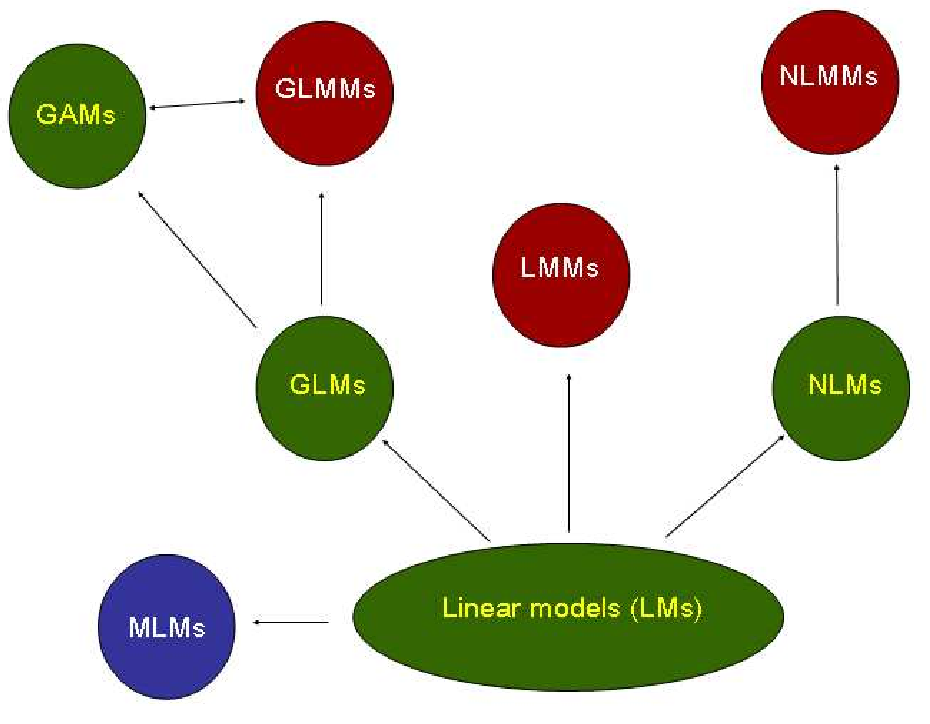
\includegraphics[scale = 0.20]{13_glmDiagram}\\
    \begin{footnotesize}
      \begin{tabular}{lll}
        \hline
        Model & Acronym & R function \\
        \hline
        \color{darkgreen}Linear Models             & \color{darkgreen}LM   & \color{darkgreen}\texttt{lm}, \texttt{aov}\\
        \color{darkblue}Multivariate LMs           & \color{darkblue}MLM   & \color{darkblue}\texttt{manova} \\
        \color{darkgreen}Generalized LMs           & \color{darkgreen}GLM  & \color{darkgreen}\texttt{glm} \\
        \color{circlered}Linear Mixed Models       & \color{circlered}LMM  & \color{circlered}\texttt{lme}, \texttt{aov} \\
        \color{darkgreen}Non-linear Models         & \color{darkgreen}NLM  & \color{darkgreen}\texttt{nls} \\
        \color{circlered}Non-linear Mixed Models   & \color{circlered}NLMM & \color{circlered}\texttt{nlme} \\
        \color{circlered}Generalized LMMs          & \color{circlered}GLMM & \color{circlered}\texttt{glmmPQL} \\
        \color{darkgreen}Generalized Additive Ms   & \color{darkgreen}GAM  & \color{darkgreen}\texttt{gam} \\
        \hline
      \end{tabular} 
    \end{footnotesize}
  \end{center}
\end{frame}



%%%%%%%%%%%%%%%%%%%%%%%%%%%%%%%%%%%%%%%%%%%%%%%%%%%%%%%%%%%%%%%

\livelloA{Generalized Linear Model (GLM)}



\livelloB{GLM: example 1}

\begin{frame}
  \begin{itemize}
    \item Collett (1991, p. 75) reports an experiment on the toxicity to the tobacco budworm Heliothis virescens of doses of the pyrethroid trans-cypermethrin to which the moths were beginning to show resistance. 
    \item Batches of 20 moths of each sex were exposed for three days to the pyrethroid and the number in each batch that were dead or knocked down was recorded.
    \item The results were\\
      \begin{center}
        \begin{tabular}{lcccccc}
          \hline
          & \multicolumn{6}{c}{Dose ($\mu$g)} \\
          \hline
          Sex & 1&2&4&8&16&32\\
          \hline
          Male&1&4&9&13&18&20\\
          Female&0&2&6&10&12&16\\
          \hline
        \end{tabular}        
      \end{center}
  \end{itemize}
\end{frame}



\livelloB{GLM: example 2}

\begin{frame}
  \begin{itemize}
    \vspace{0.5cm}
    \item An experiment recorded the numbers of chromosomal abnormalities observed for various amounts and intensities of gamma radiation.
    \vspace{0.5cm}
    \item The number of cells per measurement varied.
    \vspace{0.5cm}
    \item The results contains, for each one of 27 measurements:
      \begin{itemize}
        \item the number of cells per measurement;
        \vspace{0.25cm}
        \item the numbers of chromosomal abnormalities;
        \vspace{0.25cm}
        \item the amount of gamma radiation;
        \vspace{0.25cm}
        \item the intensity of gamma radiation.   
      \end{itemize}
  \end{itemize}
\end{frame}



\livelloB{How to specify response variable in R}

\begin{frame}
  \begin{itemize}
    \vspace{0.5cm}
    \item In the case of binomial data, response variable may be specified in three different ways:
      \begin{enumerate}
        \vspace{0.25cm}
        \item If the response is a numeric vector it is assumed to hold the data in ratio form, $ y_i = s_i / a_i $, in which case the $a_i$s must be given as a vector of weights using the \texttt{weights} argument. If the $ a_i $ are all one, the default \texttt{weights} suffices.
        \vspace{0.25cm}
        \item If the response is a logical vector or a two-level factor it is treated as a 0/1 numeric vector and handled as previously.
        \vspace{0.25cm}
        \item If the response is a two-column matrix it is assumed that the first column holds the number of successes, $ s_i $, and the second holds the number of failures, $ a_i - s_i $, for each trial. In this case, no \texttt{weights} argument is required.
      \end{enumerate}
  \end{itemize}
\end{frame}



\livelloB{Introduction}

\begin{frame}
  \begin{itemize}
    \item Generalized Linear Models (\textbf{GLM}) are extensions of fixed-effects linear model to cases where standard linear model assumptions are violated.
    \item Standard linear model:
      $$ y_i = \beta_0 + \beta_1 \cdot x_{i1} + \beta_2 \cdot x_{i2} + \dots + \beta_p \cdot x_{ip} + \varepsilon_i $$

      The above formula can be written in a matrix format:
      $$ \vect{y} = \matr{X} \vect{\beta} + \vect{\varepsilon} $$

      or, in terms of expected values:
      $$ E(\vect{y}) = \matr{X} \vect{\beta} $$

      Estimation is done by least squares, based on the assumption of normal errors. 
  \end{itemize}
\end{frame}

\begin{frame}
  \begin{itemize}
    \vspace{0.5cm}
    \item GLM uses a likelihood-based procedure to fit $ \matr{X} \vect{\beta} $ to a function of $ E(\vect{y}) $, suggested by the distribution of data.
    \vspace{0.5cm}
    \item $ \vect{y} $ is described as an additive function of \textbf{systematic} and \textbf{random} components. The first corresponds to $ E(\vect{y}) $, the later to error.
      $$ \vect{y} = \vect{\mu} + \vect{\varepsilon} $$
      \begin{itemize}
        \item $ Var(\vect{y}) = Var(\vect{\varepsilon}) = R $.
        \vspace{0.2cm}
        \item $ \vect{\eta} = \matr{X} \vect{\beta}$, where $ \vect{\eta} = g(\vect{\mu}) $.
        \vspace{0.2cm}
        \item $ g(\vect{\mu}) $ is called the \textbf{link function}, because it links the linear model to the mean of $ \vect{y} $.
      \end{itemize}
  \end{itemize}
\end{frame}

\begin{frame}
  \begin{itemize}
    \item Nelder and Wedderburn (1972) showed that the Maximum Likelihood Estimates (MLEs) for $ \vect{\beta} $ can be obtained iteratively solving:
      $$ \matr{X^T} \matr{W} \matr{X} \matr{\beta} =  \matr{X^T} \matr{W} \matr{y^*} $$
      with
      \begin{itemize}
        \item $ \matr{W} = \matr{D} \matr{R^{-1}} \matr{D} $
        \item $ \vect{y^*} = \vect{\hat{\eta}} + (\vect{y} - \vect{\tilde{\mu}}) \matr{D^{-1}} $
        \item $ \vect{D} = \partial \vect{\mu} / \partial \vect{\eta} $
        \item $ \matr{R} = Var(\vect{\varepsilon}) $
        \item $ \vect{\mu} = E(\vect{y}) $
      \end{itemize}
    \vspace{0.25cm}
    \item Estimates of $ \matr{D} $ and $ \matr{R} $ are used in place of $ \matr{D} $ and $ \matr{R} $.
    \vspace{0.25cm}
    \item In the case of standard linear model, $ \vect{\eta} = E(\vect{y}) = \vect{\mu} $ and $ \matr{D} = \matr{I} $. Thus, $ \matr{X^T} \matr{R^{-1}} \matr{X} \matr{\beta} =  \matr{X^T} \matr{R^{-1}} \matr{y} $, the normal equation.
  \end{itemize}
\end{frame}



\livelloB{Probability distribution}

\begin{frame}
  \begin{itemize}
    \vspace{0.75cm}
    \item Elements for estimating $ \vect{\beta} $:
      \begin{itemize}
        \vspace{0.25cm}
        \item \textbf{link function}: determines $ \vect{\nu} $ and $ \matr{D} $;
        \vspace{0.25cm}
        \item \textbf{probability function}: determines $ \vect{\mu} $ and $ \matr{R} $.
      \end{itemize}
    \vspace{0.5cm}
    \item The process for selecting a link function and the structure of the mean and variance can be understood by looking at the probability distribution, or, better said, to the likelihood function.
    \vspace{0.5cm}
    \item Three cases will be considered: the Binomial, the Poisson and the Normal.
  \end{itemize}
\end{frame}



\livelloB{The Binomial case}

\begin{frame}
  \begin{itemize}
    \item $ n $ trials, each trial with succes probability of $ \pi $:
      $$ f(y_{n}) = \binom{n}{y_{n}} \pi^{y_n} (1-\pi)^{n-y_{n}} $$
    \vspace{0.075cm}
    \item The log-likelihood function is:
      $$ l(\pi; y_{n}) = y_{n} \log \left(\frac{\pi}{1-\pi}\right) + n \log(1-\pi) + \log \binom{n}{y_{n}} $$
    \vspace{0.075cm}
    \item A sample proportion, $ y = y_{n}/n $, thus has a log-likelihood function of
      $$ l(\pi; y_{n}) = n y_{n} \log \left(\frac{\pi}{1-\pi}\right) + n \log(1-\pi) + \log \binom{n}{ny_{n}} $$
    \vspace{0.075cm}
    \item Mean and variance of a sample proportion are:
      $$ E(y) = \pi \hspace{2cm} Var(y) = \frac{\pi (1-\pi)}{n} $$
  \end{itemize}
\end{frame}



\livelloB{The Poisson case}

\begin{frame}
  \begin{itemize}
    \item The probability function of the Poisson distribution is:
      $$ f(y) = \frac{\lambda^y e^{-\lambda}}{y!} $$
    \vspace{0.1cm}
    \item The log-likelihood function is:
      $$ l(\lambda; y) = y \log(\lambda) - \lambda - \log(y!) $$
    \vspace{0.1cm}
    \item Mean and variance  are:
      $$ E(y) = \lambda \hspace{2cm} Var(y) = \lambda $$
  \end{itemize}
\end{frame}



\livelloB{The Normal case}

\begin{frame}
  \begin{itemize}
    \item The probability function of the Normal distribution is:
      $$ f(y) = \frac{1}{\sqrt{2\pi\sigma^2}} \exp{\left(-\frac{1}{2\sigma^2}(y-\mu)^2\right)} $$
    \vspace{0.1cm}
    \item The log-likelihood function is:
      $$ l(\mu, \sigma^2; y) = \left(-\frac{1}{2\sigma^2}\right) (y-\mu)^2 - \frac{1}{2} \log(2\pi\sigma^2) $$
    \vspace{0.1cm}
    \item Mean and variance  are:
      $$ E(y) = \mu \hspace{2cm} Var(y) = \sigma^2 $$
  \end{itemize}
\end{frame}



\livelloB{Common features}

\begin{frame}
  \begin{itemize}
    \item The log-likelihood functions for these three distributions have a common form,
      $$ l(\theta, \phi; y) = \frac{y\theta - b(\theta)}{a(\phi)} + c(y, \phi) $$
      where
      \begin{itemize}
        \item $ \theta $ is the natural parameter,
        \item $ \phi $ is the scale parameter.
      \end{itemize}
    \vspace{0.2cm}
    \item $ \theta $ is a function of the mean, $ \theta(\mu) $. 
    \vspace{0.2cm}
    \item It is also possible express the variance as a function of the mean and $ a(\phi) $:
      $$ Var(y) = V(\mu)a(\phi) $$
      where $ V(\mu) $ is the \textbf{variance function}.
  \end{itemize}
\end{frame}

\begin{frame}
  \vspace{1.6cm}
  \begin{table}
    \begin{tabular}{c|ccc}
      \hline
      & Sample proportion & Poisson & Normal\\
      \hline
      $ E(y) $        & $ \pi $               & $ \lambda $       & $ \mu $      \\
      $ \theta(\mu) $ & $ \log(\pi/(1-\pi)) $ & $ \log(\lambda) $ & $ \mu $      \\
      $ a(\phi) $     & $ 1/n $               & $ 1 $             & $ \sigma^2 $ \\
      $ V(\mu) $      & $ \pi(1-\pi) $        & $ \lambda $       & $ 1 $        \\
      $ Var(y) $      & $ \pi(1-\pi)/n $      & $ \lambda $       & $ \sigma^2 $ \\
      \hline
    \end{tabular}
  \end{table}
\end{frame}



\livelloB{Exponential family of distributions}

\begin{frame}
  \begin{itemize}
    \item A distribution whose log-likelihood has the general form
      $$ l(\theta, \phi; y) = \frac{y\theta - b(\theta)}{a(\phi)} + c(y, \phi) $$
      is a member of the \textbf{exponential family}.
    \item The GLM can be applied to data distributed according to the exponential family.
    \item If $ y_1, \dots, y_n $ is a random sample from such a family, the log-likelihood of $ y_i $ is
      $$ l(\theta_i, \phi_i; y_i) = \frac{y_i\theta_i - b(\theta_i)}{a(\phi_i)} + c(y_i, \phi_i) $$
    \item The joint log-likelihood of $ y_1, \dots, y_n $ is
      $$ l(\vect{\theta}, \vect{\phi}; y_1, \dots, y_n) = \sum_i \frac{y_i\theta_i - b(\theta_i)}{a(\phi_i)} + c(y_i, \phi_i) $$
  \end{itemize}
\end{frame}



\livelloB{Link functions and variance structure}

\begin{frame}
  \begin{itemize}
    \vspace{0.75cm}
    \item Observations are linear in the \textbf{natural parameter} $ \theta $.
      \begin{itemize}
        \vspace{0.25cm}
        \item For normally distributed data: $ \theta = \mu $.
        \vspace{0.25cm}
        \item For Poisson distributed data: $ \theta = \log(\lambda) $.
        \vspace{0.25cm}
        \item For Binomial distributed data: $ \theta = \log(\pi/(1-\pi)) $.
      \end{itemize}
    \vspace{0.75cm}
    \item In these examples, $ \theta(\mu) $ is used as a link function, they are called the \textbf{canonical link functions}.
  \end{itemize}
\end{frame}



\livelloB{Variance structure}

\begin{frame}
  \begin{itemize}
    \vspace{0.75cm}
    \item The structure of the variance-covariance matrix of $ \vect{y} $, or errors, can be described in terms of the scale parameter and variance function. Specifically,
      $$ Var(\vect{\varepsilon}) = \matr{R} = \matr{R_\mu^{1/2}} \matr{A} \matr{R_\mu^{1/2}} $$
      where
      \begin{itemize}
        \vspace{0.25cm}
        \item $ R_\mu $ is the diagonal matrix whose $i$-th diagonal element is $ V(\mu_i) $, the variance function for the $i$-th observation;
        \vspace{0.25cm}
        \item $ R_\mu^{1/2} $ is the diagonal matrix of square roots of the corresponding elements of $ R_\mu $;
        \vspace{0.25cm}
        \item $ A $ is the scale parameter matrix.
      \end{itemize}
  \end{itemize}
\end{frame}

\begin{frame}
  \vspace{1.9cm}
  \begin{table}
    \begin{tabular}{c|cc}
      \hline
      Distribution & $ \matr{R_\mu} $ & $ \matr{A} $ \\
      \hline
      Normal            & $ \matr{I} $                      & $ \matr{I_{\sigma^2}} $ \\
      Poisson           & $ \text{diag}(\lambda_i) $        & $ \matr{I} $            \\
      Sample proportion & $ \text{diag}(\pi_i/(1-\pi_i)) $  & $ \text{diag}(1/n_i) $        \\
      \hline
    \end{tabular}
  \end{table}
\end{frame}



\livelloB{Predicting means}

\begin{frame}
  \begin{itemize}
    \vspace{0.15cm}
    \item The \textbf{inverse link function} (sometimes referred to as the \textbf{mean function}) is defined as $ h(\eta) = \vect{\mu} $.
    \vspace{0.25cm}
    \item It can be used to predict $ \vect{\mu} $ from $ \vect{\hat{\beta}} $. 
    \vspace{0.25cm}
    \item It is assumed that the relationship between $ \vect{\eta} $ and $ \vect{\mu} $ is one-to-one, thus $ h(\eta) = g^{-1}(\eta) $. For some complex GLMs, this may be false.
    \vspace{0.25cm}
    \item Because $ \vect{\eta} $ is estimated by $ \matr{X}\matr{\hat{\beta}}$, $ \hat{\mu} = h(\matr{X}\vect{\hat{\beta}}) $.
      \begin{itemize}
        \vspace{0.15cm}
        \item Normal: \\
          \hspace{1cm} $ \eta = \mu \Rightarrow \mu = h(\matr{X}\vect{\hat{\beta}}) = \matr{X}\vect{\hat{\beta}} $
        \vspace{0.15cm}
        \item Poisson: \\
          \hspace{1cm} $ \eta = \log{\lambda} \Rightarrow \lambda = h(\matr{X}\vect{\hat{\beta}}) = \exp{\matr{X}\vect{\hat{\beta}}} $
        \vspace{0.15cm}
        \item Sample proportion: \\
          \hspace{1cm} $ \eta = \log{(\pi/(1-\pi))} \Rightarrow \lambda = h(\matr{X}\vect{\hat{\beta}}) = \exp{\matr{X}\vect{\hat{\beta}}}/(1+\exp{\matr{X}\vect{\hat{\beta}}}) $ \\
      \end{itemize}
  \end{itemize}
\end{frame}



\livelloB{Deviance}

\begin{frame}
  \begin{itemize}
    \item Deviance is defined as:
      $$ Dev(\vect{\hat{\mu}};\vect{y}) = 2\left(l(\vect{y};\vect{y}) - l(\vect{\hat{\mu}};\vect{y})\right) $$
      where
      \begin{itemize}
        \item $ l(y;y) $ is the value of the maximum log-likelihood achievable in a full model; i.e. it is the value of the log-likelihood for which $ \theta $ is expressed as a function of $ y $;
        \item $ l(\hat{\mu};y) $ is the value of the log-likelihood over $ \beta $, i.e. it is the vale of the log-likelihood for which $ \theta $ is expressed as a function of $ \hat{\mu} $.
      \end{itemize}
    \item The deviance is a generalization of the Sum of Squares for Error in the Analysis of Variance and the likelihood ratio $ \chi^2 $ in contingency tables:
%        \begin{itemize}
%         \vspace{0.15cm}
%         \item $ Dev \equiv SS_{ERROR} $ for normal errors;
%         \item $ Dev \equiv \text{LR } \chi^2 $ for Poisson errors.
%       \end{itemize}
    \item Deviance can be used to:
       \vspace{-0.15cm}
       \begin{itemize}
        \item evaluate \textbf{goodness-of-fit};
        \item \textbf{test hypotheses}.
      \end{itemize}
  \end{itemize}
\end{frame}



\livelloB{Goodness-of-fit}

\begin{frame}
  \begin{itemize}
    \vspace{0.5cm}
    \item $ Dev $ is a function of $ \theta $ and $ \phi $.
    \vspace{0.5cm}
    \item When $ \phi $ is known then:
      \begin{itemize}
        \item $ Dev \sim \chi^2(n-p) $ where $ n $ is the number of observations and $ p $ is the number of parameters in $ \vect{\beta} $ (including intercept, if any);
        \item therefore, $ Dev $ can be used as a $ \chi^2 $ statistics to test the goodness-of-fit (GOF) of the model.
      \end{itemize}
    \vspace{0.5cm}
    \item When $ \phi $ is unknown, it can be estimated and used to compute the \textbf{scaled deviance}:
      $$ Dev^*(\vect{\hat{\mu}};\vect{y}) = Dev(\vect{\hat{\mu}};\vect{y})/\hat{\phi} $$
  \end{itemize}
\end{frame}



\livelloB{Hypotheses testing}

\begin{frame}
  \begin{itemize}
    \item If $ \vect{\beta} $ is partitioned in $ \vect{\beta_1} $ and $ \vect{\beta_2} $ then
      $$ \matr{X}\vect{\beta} = \matr{X_1}\vect{\beta_1} + \matr{X_2}\vect{\beta_2} $$
    \vspace{0.25cm}
    \item The difference between the deviance of the full model and that of the model fitting $ \matr{X_1}\vect{\beta_1} $ ca be used as likelihood ratio (LR) to test
      $$ H_0: \vect{\beta_2} = \vect{0} $$
      $$ LR \sim \chi^2{p-p_1} $$
      where $ p_1 $ is the number of parameters in $ \vect{\beta_1} $.
    \vspace{0.25cm}
    \item When $ \phi $ is unknown, the scaled difference can be used to test hypotheses.
  \end{itemize}
\end{frame}



\livelloB{Inference using estimable functions}

\begin{frame}
  \begin{itemize}
    \item It can be shown that 
      $$ Var(\vect{\beta}) = \left( \matr{X^T} \matr{W} \matr{X} \right)^{-1} $$ 
      then
      $$ Var \left( \matr{K^T} \vect{\beta} \right) = \matr{K^T} \left( \matr{X^T} \matr{W} \matr{X} \right) \matr{K} $$
      where $ \matr{K^T} \vect{\beta} $ is an estimable function.
    \vspace{0.1cm}
    \item The \textbf{Wald statistic} for $ H_0 = \matr{K^T} \vect{\beta} = \matr{K^T} \vect{\beta_0} $ is
      $$ \left( \matr{K^T} \vect{\beta} - \matr{K^T} \vect{\beta_0} \right)^T \left[ \matr{K^T} \left( \matr{X^T} \matr{W} \matr{X} \right)^{-1} \matr{K} \right] \left( \matr{K^T} \vect{\beta} - \matr{K^T} \vect{\beta_0} \right) $$
    \item The scalar form of the Wald statistic is
      $$ \frac{\beta - \beta_0}{Var(\beta - \beta_0)} $$
    \item The Wald statistic is distributed as a $ \chi^2_{\nu} $ where $ \nu = \text{rank}(\matr{K}) $.
  \end{itemize}
\end{frame}



\livelloB{Residual diagnostics}

\begin{frame}
  \begin{itemize}
    \vspace{0.75cm}
    \item Residuals are computed as in the linear model:
      $$ r_i = y_i - \hat{y}_i $$
    \vspace{0.25cm}
    \item Residual diagnostic test the fulfillment of the assumptions of the generalized linear model:
      \begin{enumerate}
        \vspace{0.5cm}
        \item testing the assumption of homogeneity of error variance;
        \vspace{0.5cm}
        \item testing for outliers.
      \end{enumerate}
  \end{itemize}
\end{frame}

\begin{frame}
  \begin{itemize}
    \vspace{0.75cm}
    \item The assumption of homogeneity of error variance can be performed with the Levene's test.
    \vspace{0.5cm}
    \item Levene's test is performed by computing:
      $$ Z_{ij} = |y_{ij} - E(y_{.j})| $$
      and then computing an F test on the $ j $ groups.
    \vspace{0.5cm}
    \item A nonsignificant result indicates no heteroskedasticity.
  \end{itemize}
\end{frame}

\begin{frame}
  \begin{itemize}
    \vspace{0.75cm}
    \item Outliers can be detected:
      \begin{enumerate}
        \item Look for standardized residuals greater than 3.5 or less than -3.5
        \item and look for high Cook's $ D $, greater than $ 4p/(n-p-1) $. For instance, if $ n = 100 $, $ p = 5 $ then high Cook's $ D $ are higher than $ 4 \cdot 5 / (100-5-1) = 20/94 $.
      \end{enumerate}
    \vspace{0.5cm}
    \item Standardized residuals are computed by 
      $$ \frac{r_i - \hat{\mu}_r}{\hat{\sigma}_r} $$
      where $ \hat{\mu}_r $ and $ \hat{\sigma}_r $ are the mean and the standard deviation of $ r_i $, respectively. 
  \end{itemize}
\end{frame}

\begin{frame}
  \begin{itemize}
    \vspace{0.75cm}
    \item Cook's $ D $ are computed by
      $$ \text{Cook's }D_i = \left(\frac{1}{p}\right)\left(\frac{h_{ii}}{1-h_{ii}}\right)\left(\frac{r_i^2}{\hat{\sigma}^2\cdot(1-h_{ii})}\right) $$
      where $ h_{ii} $ is the $i$-th diagonal entry of the hat matrix $ \matr{H} $.
    \vspace{0.75cm}
    \item Cook and Weisberg (1982) suggested that values of $ D_i $ that exceed 50\% of the $ F $ distribution with $ p $ and $ n-p $ degrees of freedom are large
  \end{itemize}
\end{frame}

\begin{frame}
  \begin{itemize}
    \item The hat matrix $ \matr{H} $ transforms $ \matr{Y} $ into the predicted scores. It is computed by
      $$ \matr{H} = \matr{X}(\matr{X}^T \matr{X})^{-1}\matr{X}^T $$
    \item The diagonals for the hat matrix indicate which values could be outliers or not.
    \item The diagonals are therefore measures of leverage.
    \item Leverage is bounded by two limits: $ 1/n $ and $ 1 $. The closer the leverage is to unity, the more levarage the value has.
    \item The trace of the hat matrix is equal to the number of variables in the model.
    \item When the leverage is greater than $ 2p/n $ ther is high leverage according to Belsley et al. (1980), cited in Long J.F., Modern Methods in Data Analysis (page 262). For smaller samples, Vellman and Welsch (1981) suggested that $3p/n$ is the criterion.
  \end{itemize}
\end{frame}

\begin{frame}
  \begin{itemize}
    \vspace{0.75cm}
    \item The leverage of outliers can be assessed:
      \begin{itemize}
        \vspace{0.25cm}
        \item constructing and analyzing studentized residuals;
        \vspace{0.25cm}
        \item constructing and analyzing the leverage of the high and low studentized residuals;
        \vspace{0.25cm}
        \item using Cook's $ D $ to help determine how problematic outliers are.
      \end{itemize}
    \vspace{0.5cm}
    \item Studentized residuals are computed by
      $$ \frac{r_i}{\hat{\sigma} \sqrt{1-h_{ii}}} $$
  \end{itemize}
\end{frame}



%%%%%%%%%%%%%%%%%%%%%%%%%%%%%%%%%%%%%%%%%%%%%%%%%%%%%%%%%%%%%%%

\livelloA{Generalized Linear Mixed Model (GLMM)}

\livelloB{Quasi-likelihood function}

\begin{frame}
  \begin{itemize}
    \item A Generalized Linear Mixed Model (GLMM) is an extension to the GLM in which the linear predictor contains random effects in addition to the usual fixed effects.
    \vspace{0.1cm}
    \item A GLMM use the \textbf{quasi-likelihood}, an extension of likelihood methods.
    \item The quasi-likelihood function is defined as follows.
      \begin{itemize}
        \item Given $ n $ observation $ y_i $ ($ i = 1, \dots, n $) such that $ E(y_i) = \mu_i $, $ Var(y_i) \propto Var(\mu_i) $ (known function), $ \mu = function(\beta_1, \dots, \beta_p) $ the quasi-likelihood function is defined by
         $$ \frac{\partial Q(\mu_i, y_i)}{\partial \mu_i} = \frac{y_i - \mu_i}{Var(\mu_i)} $$
        \item An example of $ \mu = function(\beta_1, \dots, \beta_p) $ is given by $ \mu_i = h(\eta_i) $, $ \eta_i = \sum_j X_{ij} \beta_j $, that is the inverse link function of a GLM
        \item The log-likelihood function is a special case of $ Q(\mu_i, y_i) $.
      \end{itemize}
  \end{itemize}
\end{frame}



\livelloB{Conditional distribution}

\begin{frame}
  \begin{itemize}
    \vspace{0.75cm}
    \item In the normal errors mixed model $ \vect{y} = \matr{X} \vect{\beta} + \matr{Z} \vect{u} + \vect{e} $
      \begin{itemize}
        \vspace{0.25cm}
        \item the conditional mean of the observations given the random model effects is $ E(\vect{y}|\vect{u}) = \mu = \matr{X} \vect{\beta} + \matr{Z} \vect{u} $,
        \vspace{0.25cm}
        \item the conditional variance is $ Var(\vect{y}|\vect{u}) = \matr{R} = Var(\vect{e}) $.
      \end{itemize}
    \vspace{0.75cm}
    \item Observation can be described as $ \vect{y} = \vect{\mu} + \vect{e} $ where $ \vect{\mu} $ is the conditional mean, $ E(\vect{y}|\vect{u}) $, $ u \sim MVN(\vect{0}, \matr{G})$. 
  \end{itemize}
\end{frame}

\begin{frame}
  \begin{itemize}
    \vspace{0.75cm}
    \item In the generalized linear mixed model, the \textbf{conditional distribution} of $ \vect{y}|\vect{u} $ plays the same role as the distribution of $ \vect{y} $ in the fixed effects generalized linear model.
    \vspace{0.75cm}
    \item The \textbf{conditional quasi-likelihood} of an observation, $ \vect{y_i}|\vect{y} $ is
      $$ Q(u_i, y_i|u_i) = \left[ \frac{y_i \theta_i - b(\theta_i)}{a(\phi_i)} \right] $$
  \end{itemize}
\end{frame}

\begin{frame}
  \begin{itemize}
    \vspace{0.75cm}
    \item The \textbf{joint quasi-likelihood} of an observation, $ \vect{y_i}|\vect{y} $ of the observations, $ \vect{y} $, is the sum of the quasi-likelihood of $ \vect{y}|\vect{u} $ and $ \vect{u} $. In matrix terms, the joint quasi-likelihood is
      $$ Q(\vect{\mu}, \vect{u}; \vect{y}) = \left[ \vect{y^T} \matr{A^{-1}} \vect{\theta} - (\vect{b_{\theta}^{1/2}})^T \matr{A^{-1}} \vect{b_{\theta}^{1/2}}) \right] + \frac{1}{2} \vect{u^T} \matr{G^{-1}} \vect{u} $$
      where:
      \begin{itemize}
        \vspace{0.25cm}
        \item $ \matr{A} $ is the matrix of $ a(\phi_i) $,
        \vspace{0.25cm}
        \item $ \vect{\theta} $ is the vector of $ \theta(\mu_i) $,
        \vspace{0.25cm}
        \item $ \vect{b_\theta} $ is the vector of $ b(\theta_i) $.
      \end{itemize}
  \end{itemize}
\end{frame}



\livelloB{Fitting a GLMM}

\begin{frame}
  \begin{itemize}
    \vspace{0.75cm}
    \item The strategies for fitting a GLMM to $ E(\vect{y}) $ are the same as those for a GLM:
    \begin{itemize}
      \vspace{0.25cm}
      \item the form of the conditional quasi-likelihood determines the \textbf{variance structure} and contains the natural parameter,
      \vspace{0.25cm}
      \item the conditional mean function $ \theta(\mu) $ is used a \textbf{canonical link}.
        $$ \eta = \matr{X} \vect{\beta} + \matr{Z} \vect{u} $$
        $$ \eta = g(\mu) $$
    \end{itemize}
  \end{itemize}
\end{frame}
 


\begin{frame}
  \begin{itemize}
    \vspace{0.75cm}
    \item The strategies for fitting a GLMM to $ E(\vect{y}) $ are the same as those for a GLM:
    \begin{itemize}
      \vspace{0.25cm}
      \item the form of the conditional quasi-likelihood determines the \textbf{variance structure} and contains the natural parameter,
      \vspace{0.25cm}
      \item the conditional mean function $ \theta(\mu) $ is used a \textbf{canonical link}.
        $$ \eta = \matr{X} \vect{\beta} + \matr{Z} \vect{u} $$
        $$ \eta = g(\mu) $$
    \end{itemize}
  \end{itemize}
\end{frame}






\end{document}
